\documentclass[11pt]{amsart}
%%%%%%%%%%%%%% Packages
\usepackage{amssymb,amsfonts,amsthm,amsmath}
\usepackage[english]{babel}
\usepackage[all,cmtip]{xy}
\usepackage{tikz}
\usepackage{mathtools}
\usepackage{tensor}
\usepackage{csquotes}
\usepackage[vcentermath]{youngtab}
%\usepackage{stix}
\usetikzlibrary{arrows,chains,matrix,positioning,scopes}
%\usepackage{mathrsfs}
%\usepackage[notcite,notref]{showkeys}


%%%%%%%%%%% Tikz
\makeatletter
\tikzset{join/.code=\tikzset{after node path={%
\ifx\tikzchainprevious\pgfutil@empty\else(\tikzchainprevious)%
edge[every join]#1(\tikzchaincurrent)\fi}}}
\makeatother
\tikzset{>=stealth',every on chain/.append style={join},
         every join/.style={->}}

        

%%%%%%%%%%%% Personalized commands and environments

\newcommand{\inputc}[1]{ \raisebox{-0.5\height}{\input{#1}} }
\newtheorem{theorem}{Theorem}
\newtheorem{lemma}[theorem]{Lemma}
\newtheorem{corollary}[theorem]{Corollary}
\newtheorem{definition}[theorem]{Definition}
\newtheorem{proposition}[theorem]{Proposition}
\newtheorem{remark}[theorem]{Remark}
\newtheorem{example}{Example}
%\newtheorem{theorem*}{Theorem}

\newcommand{\func}[3]{{#1} : {#2} \longrightarrow {#3}}
\numberwithin{equation}{section}
\newcommand{\dbar}{\bar{\partial}}
\newenvironment{myproof}{\noindent{it Proof}
\setlength{\parindent}{0mm}}
{$\hfill \bs$}


%%%%%%%%%%%%%%%%%%%%%%%% Title and Author information

\title{MAT 303 Recitations: Week 13}


\author[M. Gomes]{Marlon de Oliveira Gomes}
\address{Mathematics Department 3-101, Stony Brook University,
100 Nicolls Road, Math Tower, 
Stony Brook, NY, 11794, USA} \email{mgomes@math.stonybrook.edu}



%%%%%%%%%%% Text
\begin{document}

\maketitle


\section*{Section 4.1: First-order systems and applications}

A system of differential equation consists of a finite collection of differential equations in indeterminates $x_1(t), x_2(t), \cdots, x_n(t)$, depending on a parameter $t$. In this chapter, we will deal with linear systems. 

One's first encounter wiht systems of differential equations arises from higher-order scalar equations. One way of solving them is by reducing such equations to systems of first-order problems, as we shall see next. 

\begin{example}
This example is extracted from problem 4.1.3 in our textbook. Consider the third-order equation
\begin{equation*}
tx^{(3)}-2t^2x^{''}+3tx^{'}+5x=\ln(t)
\end{equation*}
By using the substitutions $x_1=x$, $x_2=x^{'}$, $x_3=x^{''}$, we can rewrite this equation as a system in three variables
\begin{align*}
tx_{3}^{'}-2t^2x_3+3tx_2+5x_1 & = \ln(t) \\
x_{2}^{'} & = x_3\\
x_1^{'} & = x_2
\end{align*}
\end{example}

\begin{example}
The following example is extracted from problem 4.1.17. Consider the system of differential equations
\begin{align*}
x^{'} & = y \\
y^{'} & = -x
\end{align*}
By elimination, we find
\begin{equation*}
x^{''} = y^{'} = -x.
\end{equation*}
This second-order equation on $x$ can be solved by the method of characteristic equations, 
\begin{equation*}
x(t)=A\cos(t)+B\sin(t).
\end{equation*}
To solve for $y$, we use the first equation in our system,  
\begin{align*}
y (t) & = x'(t) \\
& = -A\sin(t)+B\cos(t).
\end{align*}
Below is a plot of the slope field for this equation, with several solution curves outlined. 
\begin{center}
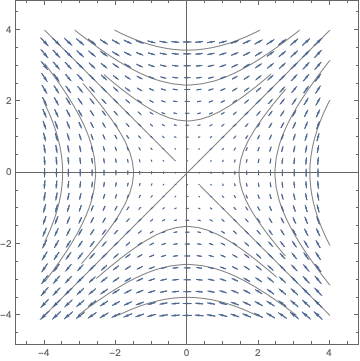
\includegraphics[width=0.5\textwidth]{p4.png} 
\end{center}
\end{example}

\begin{example}
In this example, extracted from problem 4.1.23, we have the system
\begin{align*}
x^{'} & = y \\
y^{'} & = 6x-y,
\end{align*}
with initial conditions $x(0)=1$, $y(0)=2$. We can turn this system into a second-order equation for $x$ as follows, 
\begin{equation*}
x^{''} = y^{'} = 6x-y = 6x-x^{'}, 
\end{equation*}
that is
\begin{equation*}
x^{''}+x^{'}-6x=0.
\end{equation*}
The characteristic polynomial of this equation is $r^2+r-6r=(r-2)(r+3)$, with roots $r=2, r=-3$.  The general solution takes the form
\begin{equation*}
x(t)=Ae^{2t}+Be^{-3t}
\end{equation*}
To find the appropriate values for the constants, we need to set up the intial conditions in terms of $x$. The initial condition on $y$ yields 
\begin{equation*}
x^{'}(0) = y(0) = 2,
\end{equation*}
thus we find
\begin{align*}
A+B & = 1\\
2A-3B & = 2,
\end{align*}
whose solutions are $A=1, B=0$. As a result, $x(t)=e^{2t}$, and 
\begin{equation*}
y(t) = x^{'}(t) = 2e^{2t}
\end{equation*}
Below is a plot of the direction field, as well as the solution curve corresponding to the given initial condition (in red).
\begin{center}
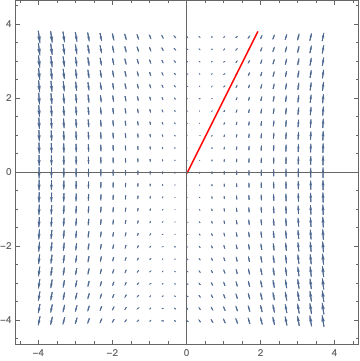
\includegraphics[width=0.5\textwidth]{p5.png} 
\end{center}
\end{example}

\section*{Section 4.2: The method of elimination}
In section 4.2 we deal with slightly more sophisticated equations for which a direct substitution is not enough to eliminate one of the variables. In such cases we will need to manipulate the equations by means of derivatives and algebraic operations to obtain the desired reduction. 
\begin{example}
Consider the following system, extracted from problem 4.2.5, 
\begin{align*}
x^{'} & = -3x-4y \\
y^{'} & = 2x+y.
\end{align*}
We will rewrite the system by using the short-hand notation $D$ to mean derivatives relative to time, $D=\frac{d}{dt}$, 
\begin{align*}
(D+3)x+4y & = 0\\
-2x + (D-1)y & = 0
\end{align*}
In order to eliminate one of the variables from the system, we will perform the following operations:
\begin{enumerate}
\item Apply the operator $(D-1)$ to the first equation, that is, differentiate it and subtract the original equation from the result.
\item Multiply the second equation by $(-4)$. 
\end{enumerate}
The resulting (equivalent) system is 
\begin{align*}
(D-1)(D+3)x+4(D-1)y & = 0\\
8x -4 (D-1)y & = 0
\end{align*}
By adding the two equations we find
\begin{equation*}
(D-1)(D+3)x + 8x =0,
\end{equation*}
which in usual notation for derivatives is 
\begin{align*}
(D-1)(D+3)x + 8x & =0\\
(D-1)(x^{'}+3x)+8x & = 0\\
(x^{'}+3x)^{'}-(x^{'}+3x)+8x & = 0\\
x^{''}+3x^{'}-x^{'}-3x+8x & = 0\\
x^{''}+2x^{'}+5x & = 0
\end{align*}
This equation can be solved by the method of characteristic equations, and we will leave the details to the reader. Its solutions take the form
\begin{equation*}
x(t)=e^{-t}(A\cos(2t)+B\sin(2t)).
\end{equation*}
To find the solution $y(t)$ we may use the first equation of the system,
\begin{align*}
y(t) & = -\frac{x^{'} +3x}{4} \\
& =-\frac{e^{-t}[(2B-A)\cos(2t) -(2A+B)\sin(2t)]+3e^{-t}(A\cos(2t)+B\sin(2t))}{4} \\
& = -\frac{e^{-t}[(A+B)\cos(2t)+(B-A)\sin(2t)]}{2}
\end{align*}
\end{example}

Lastly, we apply the method of elimination to an inhomogeneous system. 
\begin{example}
In problem 4.2.8, we are given the system
\begin{align*}
x^{'} & = 2x+y \\
y^{'} & = x+2y-e^{2t},
\end{align*}
which we rewrite in the form
\begin{align*}
(D-2)x - y & = 0 \\
-x + (D-2)y & = -e^{2t}
\end{align*}
The easier route to solve this problem is the following to apply the operator $(D-2)$ to the first equation, resulting in
\begin{align*}
(D-2)(D-2)x - (D-2)y & = 0 \\
-x + (D-2)y & = -e^{2t}.
\end{align*}
Adding the two equations we obtain
\begin{equation*}
x^{''}-4x^{'}+3x=0,
\end{equation*}
whose solutions take the form 
\begin{equation*}
x(t)=Ae^{t}+Be^{3t},
\end{equation*}
from which we find
\begin{equation*}
x^{'}(t) = Ae^{t}+3Be^{3t}.
\end{equation*}
Substituting both $x(t)$ and $x^{'}(t)$ into the first equation we compute $y(t)$:
\begin{align*}
y(t) & = x^{'}(t)-2x(t) \\
& = Ae^{t}+3Be^{3t} -2(Ae^{t}+Be^{3t}) \\
& = -Ae^{t}+Be^{3t}
\end{align*}
\end{example}
\begin{thebibliography}{0}

\bibitem{EdPeCa} C. Henry Edwards, David E. Penney and David T. Calvis, {\it Differential Equations and Boundary Value Problems: Computing and Modelling}, 5th edition, Pearson, 2014.

\end{thebibliography}
\end{document}


